\documentclass[border=10pt]{standalone}
\usepackage[svgnames]{xcolor}
\usepackage{amsmath}
\usepackage{pgfplots}
\pgfplotsset{compat=newest}
\usepackage[sfdefault]{FiraSans}
\usepackage{FiraMono}
\renewcommand*\familydefault{\sfdefault}
\begin{document}
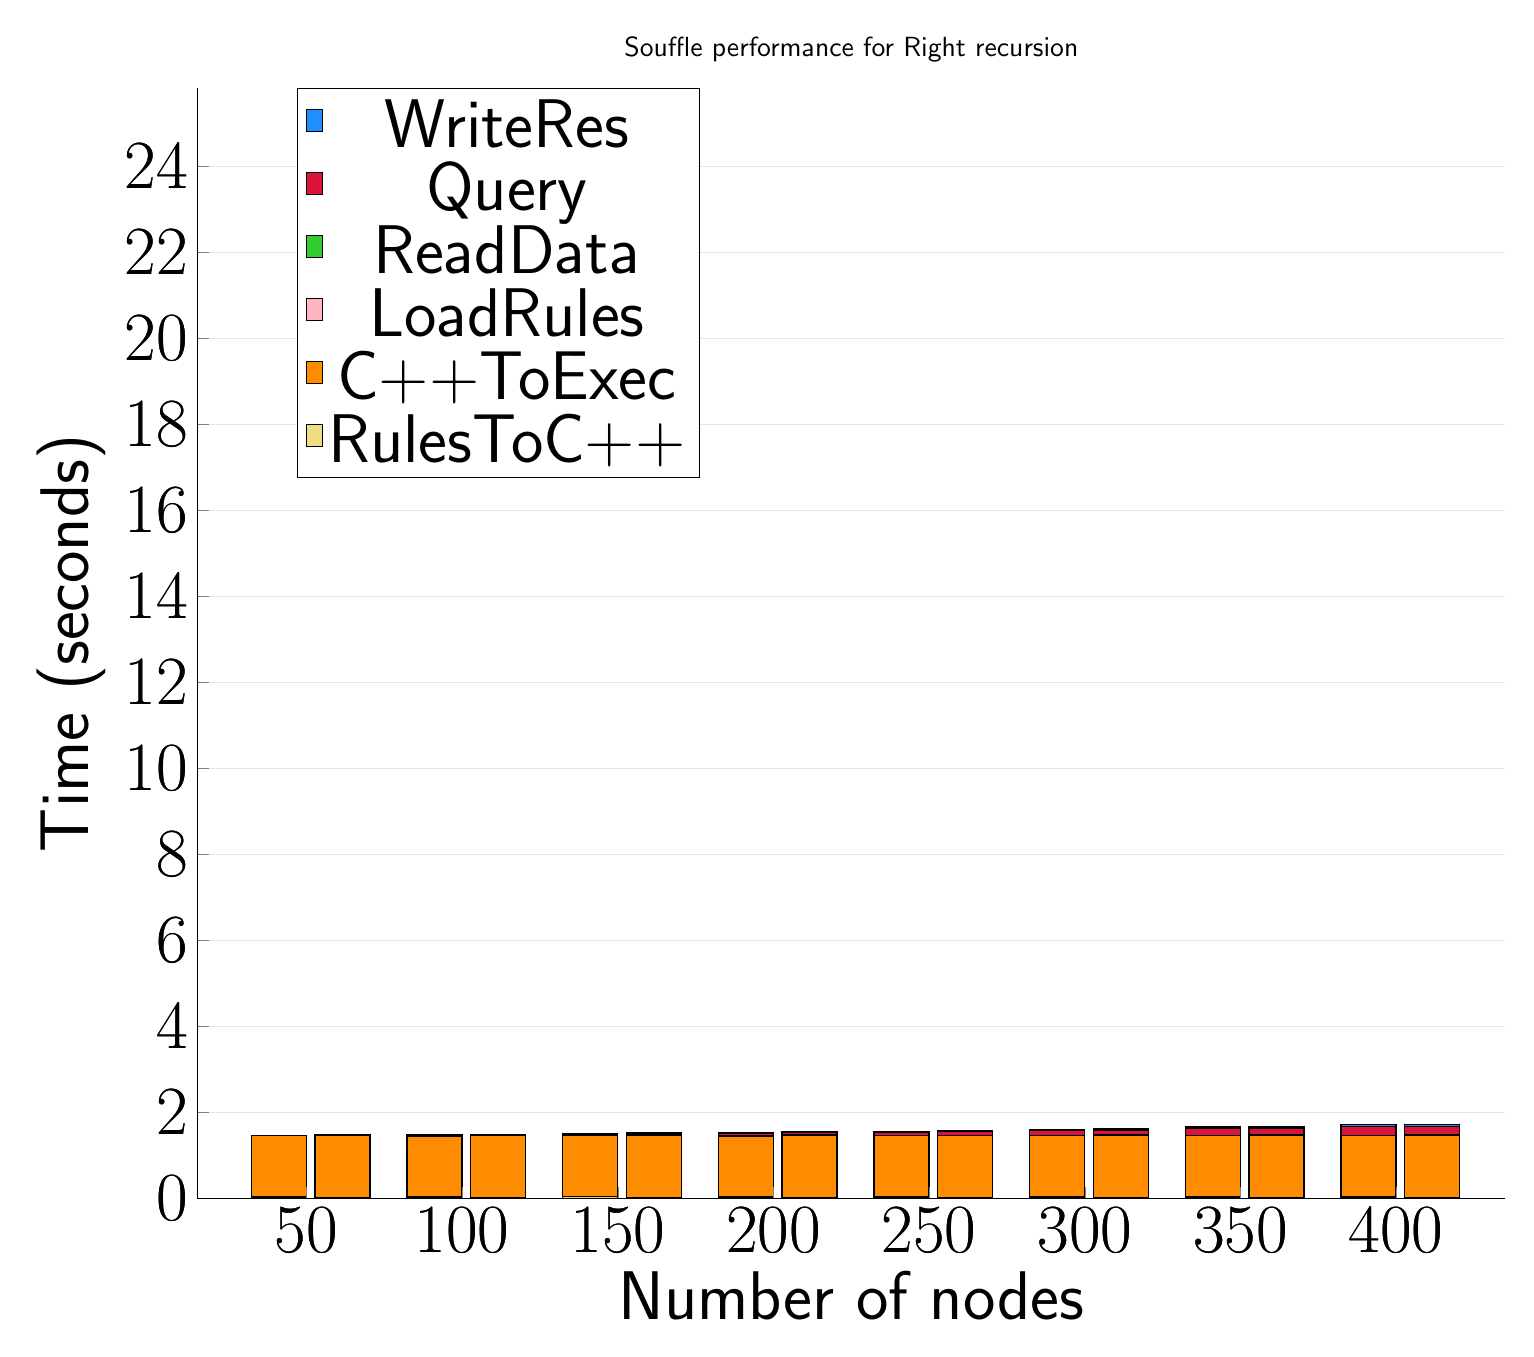
\begin{tikzpicture}
\begin{axis}[
   ybar stacked,
   title={Souffle performance for Right recursion},
   bar shift=-10pt,
   width=1.5\textwidth,
   bar width=0.7cm,
   ymajorgrids, tick align=inside,
   major grid style={draw=gray!20},
   xtick=data,
   ymin=0, ymax=25.820519999999995,
   axis x line*=bottom,
   axis y line*=left,
   enlarge x limits=0.1,
   legend style={
       at={(0.23, 1)},
       anchor=north,
       legend columns=1,
       font=\Huge,
   },
   ylabel={Time (seconds)},
   xlabel={Number of nodes},
   label style={font=\Huge},
   tick label style={font=\Huge},
]
\addlegendimage{fill=DodgerBlue, draw=black, line width=0.2pt}
\addlegendentry{WriteRes}
\addlegendimage{fill=Crimson, draw=black, line width=0.2pt}
\addlegendentry{Query}
\addlegendimage{fill=LimeGreen, draw=black, line width=0.2pt}
\addlegendentry{ReadData}
\addlegendimage{fill=LightPink, draw=black, line width=0.2pt}
\addlegendentry{LoadRules}
\addlegendimage{fill=DarkOrange, draw=black, line width=0.2pt}
\addlegendentry{C++ToExec}
\addlegendimage{fill=LightGoldenrod, draw=black, line width=0.2pt}
\addlegendentry{RulesToC++}
\addplot +[fill=LightGoldenrod, draw=black, line width=0.5pt] coordinates {
    (50, 0.039999961853027344)
    (100, 0.04000000953674317)
    (150, 0.04200003147125244)
    (200, 0.03900001049041748)
    (250, 0.04000000953674317)
    (300, 0.039999961853027344)
    (350, 0.03899998664855957)
    (400, 0.040999960899353025)
};
\addplot +[fill=DarkOrange, draw=black, line width=0.5pt] coordinates {
    (50, 1.421000075340271)
    (100, 1.419000005722046)
    (150, 1.424999976158142)
    (200, 1.418999981880188)
    (250, 1.4200000047683716)
    (300, 1.4250000715255737)
    (350, 1.427999997138977)
    (400, 1.4250000238418579)
};
\addplot +[fill=LightPink, draw=black, line width=0.5pt] coordinates {
    (50, 2.56417e-05)
    (100, 0.0)
    (150, 1.12042e-05)
    (200, 1.0124999999999999e-05)
    (250, 1.09125e-05)
    (300, 1.10666e-05)
    (350, 1.115e-05)
    (400, 1.11375e-05)
};
\addplot +[fill=LimeGreen, draw=black, line width=0.5pt] coordinates {
    (50, 0.0004289126)
    (100, 0.0005799412999999999)
    (150, 0.0006309708)
    (200, 0.0007961958)
    (250, 0.0008289122000000001)
    (300, 0.0008814458000000003)
    (350, 0.0010463029999999997)
    (400, 0.0011219995)
};
\addplot +[fill=Crimson, draw=black, line width=0.5pt] coordinates {
    (50, 0.004320170999999999)
    (100, 0.01600516)
    (150, 0.0350554)
    (200, 0.05781596)
    (250, 0.08546650999999998)
    (300, 0.11752270000000002)
    (350, 0.1595426)
    (400, 0.20621359999999997)
};
\addplot +[fill=DodgerBlue, draw=black, line width=0.5pt] coordinates {
    (50, 0.0013831085)
    (100, 0.004169244999999999)
    (150, 0.007597641)
    (200, 0.01174308)
    (250, 0.01767592)
    (300, 0.02531002)
    (350, 0.034697790000000006)
    (400, 0.04582594)
};
\end{axis}
\begin{axis}[
   ybar stacked,
   bar shift=13pt,
   width=1.5\textwidth,
   bar width=0.7cm,
   ymajorgrids, tick align=inside,
   major grid style={draw=none},
   xtick=data,
   ymin=0, ymax=25.820519999999995,
   axis x line*=none,
   axis y line*=none,
   enlarge x limits=0.1,
   label style={font=\Huge},
   tick label style={font=\Huge},
]
\addplot +[fill=LightGoldenrod, draw=black, line width=0.5pt] coordinates {
    (50, 0.031000000000000007)
    (100, 0.030000000000000006)
    (150, 0.030000000000000006)
    (200, 0.030000000000000006)
    (250, 0.030000000000000006)
    (300, 0.030000000000000006)
    (350, 0.030000000000000006)
    (400, 0.030000000000000006)
};
\addplot +[fill=DarkOrange, draw=black, line width=0.5pt] coordinates {
    (50, 1.446)
    (100, 1.4389999999999998)
    (150, 1.451)
    (200, 1.4449999999999998)
    (250, 1.4399999999999997)
    (300, 1.4460000000000002)
    (350, 1.4489999999999998)
    (400, 1.4439999999999997)
};
\addplot +[fill=LightPink, draw=black, line width=0.5pt] coordinates {
    (50, 2.5300000000000002e-05)
    (100, 0.0)
    (150, 1.11e-05)
    (200, 1.01e-05)
    (250, 1.09e-05)
    (300, 1.09e-05)
    (350, 1.1e-05)
    (400, 1.11e-05)
};
\addplot +[fill=LimeGreen, draw=black, line width=0.5pt] coordinates {
    (50, 0.0004142)
    (100, 0.0005162)
    (150, 0.0006143)
    (200, 0.0007325)
    (250, 0.0008121000000000002)
    (300, 0.0008624000000000001)
    (350, 0.0010308)
    (400, 0.0011068999999999999)
};
\addplot +[fill=Crimson, draw=black, line width=0.5pt] coordinates {
    (50, 0.0043143)
    (100, 0.0159942)
    (150, 0.03501230000000001)
    (200, 0.0576405)
    (250, 0.08530890000000001)
    (300, 0.11729890000000001)
    (350, 0.1592501)
    (400, 0.20581960000000002)
};
\addplot +[fill=DodgerBlue, draw=black, line width=0.5pt] coordinates {
    (50, 0.0013817)
    (100, 0.0039406)
    (150, 0.0074017)
    (200, 0.011368800000000002)
    (250, 0.017483199999999997)
    (300, 0.025026399999999997)
    (350, 0.0343169)
    (400, 0.045253400000000006)
};
\end{axis}
\end{tikzpicture}

\end{document}
